\graphicspath{{notes/4sets/}}
\section{Sets and Functions}\label{chap:sets}

Sets are the fundamental building blocks of mathematics. In the sub-discipline of Set Theory, mathematicians define all basic notions, including number, addition, function, etc., purely in terms of sets. In such a system it can take over 100 pages of discussion to \emph{prove} that $1+1=2$! We will not be anything like so rigorous. Indeed, before one can accept that such formality has its place in mathematics, a level of familiarity with sets and their basic operations is necessary.

\subsection{Set Notation and Describing a Set}

We start with a naïve notion: a set is a collection of objects.\footnote{For this course, our notion is enough. It eventually became clear that some collections of objects cannot be considered sets, and the search for a completely rigorous definition began; thus was Axiomatic Set Theory born.}

\begin{defn}
If $x$ is an object in a set $A$, we write $x\in A$ and say that $x$ is an \emph{element} or \emph{member} of $A$.\\
On the other hand, if $x$ is a member of some other set $B$, but not of $A$, we write $x\notin A$.\\
Sets $C$ and $D$ are described as \emph{equal,} written $C=D$, if they have exactly the same elements.
\end{defn}

\noindent\begin{minipage}{0.73\textwidth}
When thinking abstractly about sets, you may find \emph{Venn diagrams} useful. A set is visualized as a region in the plane and, if necessary, members of the set can be thought of as dots in this region. This is most useful when one has to think about multiple, possibly over-lapping, sets. The graphic represents a set $A$ with at least three elements $a_1,a_2,a_3$. The element $x$ does not lie in $A$. 
\vspace{5pt}
\end{minipage}\hfill
\begin{minipage}{0.20\textwidth}
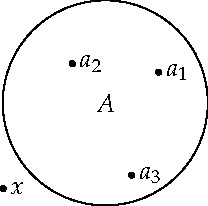
\includegraphics[width=\textwidth]{sets-01-venn}
\end{minipage}


\subsubsection*{Notation and Conventions}

We use capital letters for sets, e.g. $A,B,C,S$, and lower-case letters for elements. It is conventional, though not required, to denote an abstract element of a set by the corresponding lower-case letter: thus $a\in A$, $b\in B$, etc.\\
Curly brackets $\{\,,\,\}$ are used to bookend the elements of a set: for instance, if we wrote
\[S=\{3,5,f,\alpha,\beta\}\]
then we'd say, `$S$ is the set whose elements are 3, 5, $f$, $\alpha$ and $\beta$.'\\
The order in which we list the elements of a set is irrelevant, thus
\[S=\{\beta,f,5,\alpha,3\}=\{f,\alpha,3,\beta,5\}.\]
Listing all the elements in such a fashion is known as \emph{roster notation.}

By contrast, \emph{set-builder notation} describes the elements of a set by starting with a larger set and restricting to those elements which satisfy some property. The symbols $\mid$ or $:$ are used as a short-hand for `such that.' Which symbol you use depends partly on taste, although the context may make one clearer to read.\footnote{See Choice of Notation, below.} For example, if $S=\{3,5,f,\alpha,\beta\}$ is the set defined above, we could write,
\[\{s\in S\mid s\text{ is a Greek letter}\}=\{s\in S:s\text{ is a Greek letter}\}=\{\alpha,\beta\}\]
We would read: `The set of elements $s$ in $S$ such that $s$ is a Greek letter is the set $\{\alpha,\beta\}$.'\pagebreak

\noindent More generally, if $S$ is a set and $P$ is a propositional function whose domain is $S$, then we can define a new set
\[A:=\{s\in S:P(s)\text{ is true}\}\]

\begin{example}
Let $A=\{2,4,6\}$ and $B=\{1,2,5,6\}$. There are many options for how to write $A$ and $B$ in set-builder notation. For example, we could write
\[A=\{2n\in\Z:n=1,\,2\text{ or }3\}\quad\text{ and }\quad B=\{n\in\Z\mid 1\le n\le 6\text{ and }n\neq 3,4\}.\]
We now practice the opposite skill by converting five sets from set-builder to roster notation.
\begin{enumerate}
  \item[] $S_1=\{a\in A:a\text{ is divisible by 4}\}=\{4\}$
  \item[] $S_2=\{b\in B:b\text{ is odd}\}=\{1,5\}$
  \item[] $S_3=\{a\in A\mid a\in B\}=\{2,6\}$
  \item[] $S_4=\{a\in A:a\not\in B\}=\{4\}$
  \item[] $S_5=\{b\in B\mid b\text{ is odd and $b-1\in A$}\}=\{5\}$
\end{enumerate}
\end{example}

\noindent Take your time getting used to this notation. Can you find an alternative description in set-builder notation for the sets $S_1,\ldots,S_5$ above? It is \emph{crucial} that you can translate between various descriptions of a set or you won't be able to read much mathematics!


\subsubsection*{Sets of Numbers}

Common sets of numbers are written in the $\mathbb{B}${\scriptsize $\mathbb{LACKBOARD}$} $\mathbb{B}${\scriptsize $\mathbb{OLD}$} typeface.
\begin{itemize}\setlength{\itemsep}{0pt}
  \item[] $\N=\Z^+=\text{natural numbers}=\{1,2,3,4,\ldots\}$
	\item[] $\N_0=\mathbb{W}=\Z_0^+=\text{whole numbers}=\{0,1,2,3,4,\ldots\}$
	\item[] $\Z=\text{integers}=\{\ldots,-3,-2,-1,0,1,2,3,\ldots\}$
	\item[] $\Q=\text{rational numbers}=\{\frac mn\colon m\in\Z\text{ and }n\in\N\} =\{\frac ab\colon a,b\in\Z\text{ and }b\neq 0\}$
	\item[] $\R=\text{real numbers}$
	\item[] $\R\setminus\Q=\text{irrational numbers}$\qquad (read `$\R$ minus $\Q$')
	\item[] $\C=\text{complex numbers}=\{x+iy:x,y\in\R,\text{ where }i=\sqrt{-1}\}$
	\item[] $\Z_{\ge n}=\text{integers $\ge n$}=\{n,n+1,n+2,n+3,\ldots\}$
	\item[] $n\Z=\text{multiples of $n$}=\{\ldots,-3n,-2n,-n,0,n,2n,3n,\ldots\}$
\end{itemize}

\noindent Where there are multiple choices of notation, we will tend to use the first in the list: for example $\N_0$ is preferred to $\Z_{\ge 0}$. The use of a subscript $0$ to include zero and a superscript $\pm$ to restrict to positive or negative numbers is standard.

\begin{exs}
\quad$7\in\Z,\qquad \pi\in\R,\qquad \pi\not\in\Q,\qquad \sqrt{-5}\in\C,\qquad -e^2\in\R^-$.\\

\noindent There are often many different ways to represent the same set in set-builder notation. For example, the set of even numbers may be written in multiple ways: think about the English translations.
\begin{align*}
2\Z&=\{2n\in\Z:n\in\Z\}\tag*{(The set of integers of the form $2n$ such that $n$ is an integer)}\\
&=\{n\in\Z:\exists k\in\Z,\ n=2k\} \tag*{(The set of integers which are a multiple of 2)}\\
&=\{n\in\Z:n\equiv 0\tpmod 2\}\tag*{(The set of integers congruent to 0 modulo 2)}\\
&=\{n\in\Z:\ 2\divides n\}\tag*{(The set of integers which are divisible by 2)}
\end{align*}
Here we use both congruence and divisor notation to obtain suitable descriptions. Can you find any other ways to describe the even numbers using basic set notation?
\end{exs}

\noindent The notation $n\Z$ is most commonly used when $n$ is a natural number, but it can also be used for other $n$. For example
\[\tfrac 12\Z=\left\{\tfrac 12x:x\in\Z\right\}=\left\{m,m+\tfrac 12:m\in\Z\right\}\]
is the set of multiples of $\frac 12$ (comprising the integers and half-integers). The notation can also be extended: for example $2\Z+1$ would denote the odd integers.

\begin{aside}
\noindent{\bf Choice of Notation}

The notations $\,\mid$ and $:$ for `such that' give you leeway in case one these symbols is being used to mean something else. For example, the final expression (above) for the even numbers is much cleaner than the alternative
\[2\Z=\{n\in\Z\mid 2\mid n\}.\]
In other situations the opposite is true. In Section \ref{sec:func1} we shall consider functions. If you recall the concept of an even function from calculus, we could denote the set of such as
\[\{f:\R\to\R:\forall x,\,f(x)=f(-x)\}\qquad\text{or}\qquad\{f:\R\to\R\mid \forall x,\,f(x)=f(-x)\}.\]
In this case the latter notation is clearly superior.
\end{aside}

\begin{examples}
  \item Write the set $A=\{x\in\R:x^2+3x+2=0\}$ in roster notation.\\[5pt]
	We are looking for the set of all real number solutions to the quadratic equation $x^2+3x+2=0$. A simple factorization tells us that $x^2+3x+2=(x+1)(x+2)$, whence $A=\{-1,-2\}$.
  \item Use the set $B=\{0,1,2,3,\ldots,24\}$ to describe $C=\{n\in\Z:n^2-3\in B\}$ in roster notation.\\[5pt]
  We see that
  \[n^2-3\in B\iff n^2\in\{3,4,5,\ldots,25,26,27\}\]
  Since $n$ must be an integer in order to be an element of $C$, it follows that
  \[C=\{\pm 2,\pm 3,\pm 4,\pm 5\}.\]
  \item It is often harder to convert from roster to set-builder notation, as you might be required to spot a pattern, and many choices could be available. For example, if
  \[D=\left\{\frac 16,\frac 1{20},\frac 1{42},\frac 1{72},\frac 1{110},\frac 1{156},\ldots\right\},\]
  you might consider it reasonable to write
  \[D=\left\{\frac 1{2n(2n+1)}:n\in\N\right\}.\]
  Of course the ellipses (\ldots) might not indicate that the elements of the set continue in the way you expect. For larger sets, the concision and clarity of set-builder notation makes it much preferred!
  \item Are the following sets equal?
  \[E=\{n^2+2\in\Z:\text{$n$ is an odd integer}\},\qquad F=\{n\in\Z:n^2+2\text{ is an odd integer}\}.\]
  It may help to first construct a table listing some of the values of $n^2+2$:
  \[\begin{array}{c|c|c}
  n&n^2&n^2+2\\\hline
  \pm 1&1&3\\
  \pm 3&9&11\\
  \pm 5&25&27\\
  \pm 7&49&51\\
  \pm 9&81&83\\[-5pt]
  \vdots&\vdots&\vdots
  \end{array}\]
  The set $E$ consists of those integers of the form $n^2+2$ where $n$ is an odd integer. By the table,
  \[E=\{3,11,27,51,83,\ldots\}.\]
  On the other hand, $F$ includes all those integers $n$ such that $n^2+2$ is odd. It is easy to see that
  \[n^2+2\text{ is odd}\iff n^2\text{ is odd}\iff n\text{ is odd.}\]
  Thus $F$ is simply the set of all odd integers:
  \[F=\{\pm 1,\pm 3,\pm 5,\pm 7,\ldots\}=2\Z+1.\]
  Plainly the two sets are not equal.
\end{examples}


\subsubsection*{Intervals}

\emph{Interval notation} is useful when discussing collections of \emph{real numbers.} You should be familiar from calculus with the words \emph{open} and \emph{closed} with regard to intervals. For example,
\begin{align*}
(0,1)&=\{x\in\R:0<x<1\},\tag*{(Open interval)}\\
[0,1]&=\{x\in\R:0\le x\le 1\},\tag*{(Closed interval)}\\
(0,1]&=\{x\in\R:0<x\le 1\}.\tag*{(Half-open interval)}
\end{align*}
When writing intervals with $\pm\infty$ use an open bracket at the infinite end(s): $[1,\infty)=\{x\in\R:x\ge 1\}$. This is since the symbols $\pm\infty$ do not represent real numbers and so are not members of any interval.

\begin{example}
Recall some basic trigonometry. Consider the set of solutions to the equation $\cos x=-\frac 12$ where $x$ lies in the interval $[0,4\pi]$. This set can be written in set-builder and roster notation as
\[\left\{x\in[0,4\pi]:\cos x=-\frac 12\right\}=\left\{\frac{2\pi}3,\frac{4\pi}3,\frac{8\pi}3,\frac{10\pi}3\right\}\]
\begin{center}
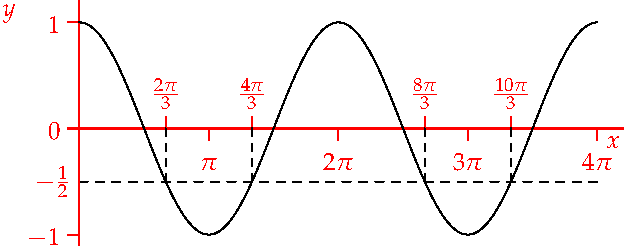
\includegraphics[width=0.6\textwidth]{sets-03-cos}
\end{center}
\end{example}

\subsubsection*{Cardinality and the Empty Set}

\begin{defn}
A set $A$ is \emph{finite} if it contains a finite number of elements: this number is the set's \emph{cardinality,} written $\nm A$. If $A$ contains infinitely many elements, it said to be an \emph{infinite set.}
\end{defn}

\begin{examples}
\item Let $A=\{a,b,\alpha,\gamma,\sqrt 2\}$, then $\nm A=5$.
\item Let $B=\Big\{4,\{1,2\},\{3\}\Big\}$. It is important to note that the \emph{elements/members} of $B$ are $4$, $\{1,2\}$ and $\{3\}$, two of which are themselves sets. Therefore $\nm B=3$. The set $\{1,2\}$ is an object in its own right, and can therefore be placed in a set along with other objects.\footnote{The fact that a set (containing objects) is also an object might seem confusing, but you should be familiar with the same problem in English. Consider the following sentences: `UCI \emph{are} constructing a laboratory' and `UCI \emph{is} constructing a laboratory.' In the first case we are thinking of UCI as a collection of individuals, in the latter case UCI is a single object. Opinions differ in various modes of English as to which is grammatically correct.}
\end{examples}

\noindent Cardinality is a very simple concept for finite sets. For infinite sets, such as the natural numbers $\N$, the concept of cardinality far much more subtle. We cannot honestly speak of $\N$ having an `infinite number' of elements, since infinity is not a number! In Chapter \ref{sec:card} we will consider what cardinality means for infinite sets and meet several bizarre and fun consequences. For the present, cardinality only has meaning for finite sets.\\

To round things off we need a symbol to denote a set that contains nothing at all!

\begin{axiom}
There exists a set $\emptyset$ with no elements (cardinality zero: $\nm\emptyset=0$). We call $\emptyset$ the \emph{empty set.}
\end{axiom}

\noindent There are many \emph{representations} of the empty set. For example $\{x\in\N:x^2+3x+2=0\}$ and $\{n\in\N:n<0\}$ are both empty. Despite this, we will see in Theorem \hyperlink{thm:subsettranslnk}{\ref*{thm:subsettrans}} that there is only one set with no elements, so that all representations actually denote the \emph{same set} $\emptyset$. 
Note also that $\nm A\in\N$ for any \emph{finite non-empty} set $A$. 

\begin{aside}
\noindent{\bf Axioms}

An axiom is a basic assumption; something that we need in order to do mathematics, but cannot prove. This is the cheat by which mathematicians can be 100\% sure that something is true: a result is proved based on the assumption of several axioms. With regard to the empty set axiom, it probably seems bizarre that we can assume the existence of some set that has nothing in it. Regardless, mathematicians have universally agreed that we need the empty set in order to do the rest of mathematics. The assumption that set-builder notation always defines a new set is another axiom.
\end{aside}

\paragraph{Self-test Questions}

\begin{enumerate}
  \item True or false: An open interval contains its endpoints.
  \item True or false: $\{x\in\R:x^2<0\}$ is a representation of the empty set.
  \item True or false: $\{x\in\Z:x\in[0,4)\}=\{0,1,2,3,4\}$.
\end{enumerate}


\subsection*{Exercises}

\begin{enumerate}\renewcommand{\labelenumi}{\thesubsection.\theenumi}
  \item Describe the following sets in roster notation: that is, list their elements.
		\begin{enumerate}
	  	\item $\{x\in\N:x^2\le 3x\}$.
	  	\item $\{x^2\in\R:x^2-3x+2=0\}$.
	  	\item $\bigl\{n+2\in\{0,1,2,3,\ldots,19\}:n+3\equiv 5\tpmod 4\bigr\}$
	  	\item $\bigl\{n\in\{-2,-1,0,1,\ldots,23\}:4\divides n^2\bigr\}$\hfill (\emph{does $:$ or  $|$ denote the condition?})
	  	\item $\{x\in \frac 12\Z: 0\le x\le 4\text{ and }4x^2\in 2\Z+1\}$
		\end{enumerate}
		
	\item Describe the following sets in set-builder notation (\emph{look for a pattern}).
		\begin{enumerate}
	  	\item $\{\ldots,-3,0,3,6,9,\ldots\}$
	  	\item $\{-3,1,5,9,13,\ldots\}$
	  	\item $\{1,\frac 13,\frac 17,\frac 1{15},\frac 1{31},\ldots\}$
	  \end{enumerate}

  \item Each of the following sets of real numbers is a single interval. Determine the interval.
		\begin{enumerate}
	  	\item $\{x\in\R:x>3\text{ and }x\le 17\}$
	  	\item $\{x\in\R:x\nleq 3\text{ or }x\le 17\}$
	  	\item $\{x^2\in\R:x\neq 0\}$
	  	\item $\{x\in\R^-:x^2\ge 16\text{ and }x^3\le 27\}$
		\end{enumerate}
		
	\item Can you describe the set $\{x\in\Z:-1\le x<43\}$ in interval notation? Why/why not?
	
	\item Compare the sets $A=\{3x\in\Z:x\in 2\Z\}$ and $B=\{x\in\Z:x\equiv 12\pmod 6\}$. Are they equal?
		
	\item What is the cardinality of the following set? What are the elements?
	\[\Bigl\{\emptyset,\bigl\{\emptyset\bigr\},\bigl\{\emptyset,\{\emptyset\}\bigr\}\Bigr\}.\]
	
	\item Let $A=\{\text{1,2,3,4}\}$, and let $B$ be the set
	\[B=\Bigl\{\{x,y\}:x,y\in A\Bigr\}.\]
	\begin{enumerate}
	  \item Describe $B$ in roster notation.
		\item Now compute the cardinality of the sets
		\[C=\Bigl\{\bigl\{x,\{y\}\bigr\}:x,y\in A\Bigr\}\]
		and
		\[D=\biggl\{\Bigl\{\bigl\{x,\{y\}\bigr\}:x,y\in A\Bigr\}\biggr\}.\]
		Compare them to $\nm B$.
	\end{enumerate}
		
  \item Prove or disprove the following conjectures.
  \begin{enumerate}
    \item $\exists x\in\R\setminus\Q$ such that $x^2\in\Q$.
    \item $\forall x\in\R\setminus\Q$ we have $x^2\in\Q$.
	\end{enumerate}
\end{enumerate}
\newpage

\subsection{Subsets}

In this section we consider the most basic manner in which two sets can be related.

\begin{defn}\label{defn:subset}
If $A$ and $B$ are sets such that every element of $A$ is also an element of $B$, then we say that $A$ is a \emph{subset} of $B$ and write $A\subseteq B$.\\
$A$ is a \emph{proper subset} of $B$ if it is a subset which is not equal. This can be written $A\subsetneq B$.\footnote{We will religiously stick to this notation. When reading other texts, note that some authors prefer $A\subset B$ for proper subset. Others use $\subset$ for any subset, whether proper or not.}
\end{defn}

\noindent The concept of subset provides us with an extremely important characterization of equality.

\begin{thm}\label{thm:setequal}
Two sets are equal if and only if they are each a subset of the other. Equivalently
\[A=B\iff A\subseteq B\text{ and }B\subseteq A.\]
\end{thm}

\begin{proof}
Recall that two sets $A$ and $B$ are equal if and only if they have the same elements. But this is if and only if every element of $A$ is also an element of $B$ and vice versa.
\end{proof}

\noindent You will often need to \emph{prove} that two sets are equal: showing that each is a subset of the other is a very common way to accomplish this.

\noindent\begin{minipage}{0.63\textwidth}
Venn diagrams are particularly useful for visualizing subset relations. The graphic on the right depicts three sets $A,B,C$: it should be clear that the only valid subset relation between the three is $A\subseteq B$.
\end{minipage}\qquad
\begin{minipage}{0.26\textwidth}
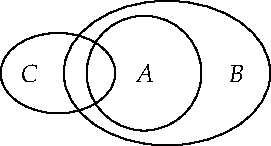
\includegraphics[width=\textwidth]{sets-02-vennsubset}
\end{minipage}\\

Set-builder notation implicitly uses the concept of subset: the notation $X=\{y\in Y:P(y)\}$ describes a set $X$ as the subset of some other set $Y$, all of whose elements satisfy the property $P(y)$. The previous section contained many examples that were subsets of the set of real numbers $\R$. Here are some other examples of subsets.

\begin{examples}
  \item $\N=\{n\in\Z:n>0\}$. This is clearly a subset of $\Z$.
  \item $\{x\in\R:x^2-1=0\}\subseteq \{y\in\R:y^2\in\N\}$.\\
  To make sense of this relationship, convert to roster notation: we obtain
  \[\{-1,1\}\subseteq\{\pm\sqrt 1,\pm\sqrt 2,\pm\sqrt 3,\pm\sqrt 4,\ldots\}.\]
  \item If $m$ and $n$ are positive integers, then $m\Z\subseteq n\Z\iff n\divides m$. Make sure you're comfortable with this! For example, $4\Z\subseteq 2\Z$ since every multiple of 4 is also a multiple of 2.
\end{examples}\pagebreak

Here we collect several results relating to subsets.

\begin{thm}\label{thm:subsettrans}\hypertarget{thm:subsettranslnk}{}
\begin{enumerate}
  \item If $\nm A=0$, then $A=\emptyset$ \hfill (Uniqueness of the empty set)
  \item For any set $A$, we have $\emptyset\subseteq A$ and $A\subseteq A$ \hfill (Trivial and non-proper subsets)
  \item If $A\subseteq B$ and $B\subseteq C$, then $A\subseteq C$\hfill(Transititvity of subsets)
\end{enumerate}%
\end{thm}

\begin{proof}
\begin{enumerate}
  \item Let $A$ be a set with cardinality zero, i.e., with no elements. $\emptyset$ has no members, therefore $\emptyset\subseteq A$ is trivial: there is nothing to check to see that all elements of $\emptyset$ are also elements of $A$! The argument for $A\subseteq\emptyset$ is identical. By Theorem \ref{thm:setequal} we see that $A=\emptyset$.
  \item Let $A$ be any set. $\emptyset\subseteq A$ follows by the argument in 1. To prove that $A\subseteq A$ we must show that all elements of $A$ are also elements of $A$. But this is completely obvious!
  \item Assume that $A$ is a subset of $B$ and that $B$ is a subset of $C$. We must show that all elements of $A$ are also elements of $C$. Let $a\in A$. Since $A\subseteq B$ we know that $a\in B$. Since $B\subseteq C$ and $a\in B$, we conclude that $a\in C$. This shows that every element of $A$ belongs to $C$. Hence $A\subseteq C$.\qedhere
\end{enumerate}
\end{proof}

As a final observation, to which we will return in Theorem \ref{thm:finitecard} and in Chapter \ref{sec:card}, your intuition should tell you that, for finite sets, subsets have smaller cardinality:
\[A\subseteq B\implies\nm A\le\nm B.\]
More generally, consider replacing the terms in Theorem \hyperlink{thm:subsettranslnk}{\ref*{thm:subsettrans}} according to the following table:
\[\begin{array}{|l|l|}\hline
\subseteq&\le\\\hline
\emptyset&0\\\hline
\text{sets }A,B,C&\text{non-negative integers}\\\hline
\text{cardinality}&\text{absolute value}\\\hline
\end{array}\]
The results should seem completely natural! Recognizing the similarities between a new concept and a familiar one, essentially spotting patterns, is perhaps the most necessary skill in mathematics.

\paragraph{Self-test Questions}

\begin{enumerate}
  \item True or false: Every set has a proper subset.
  \item Suppose that $A$ is a proper subset of $B$. What else do we need to assume about the sets $A$ and $B$ before we can say that $\nm A<\nm B$?
  \item Order the following sets of numbers according to which are subsets of which:
  \[\R,\quad \Z,\quad \N_0,\quad \N,\quad \Q,\quad \C\]
\end{enumerate}

\subsection*{Exercises}

\begin{enumerate}\renewcommand{\labelenumi}{\thesubsection.\theenumi}
  \item Let $A,B,C,D$ be the following sets.
  \begin{gather*}
  A=\{-4,1,2,4,10\}\\
  B=\{m\in\Z:\nm{m}\le 12\}\\
  C=\{n\in\Z:n^2\equiv 1\negthickspace\negthickspace\pmod 3\}\\
  D=\{t\in\Z:t^2+3\in [4,20)\}  
  \end{gather*}
  Of the 12 possible subset relations $A\subseteq B,\ A\subseteq C,\ldots D\subseteq C$, which are true and which false?
  
  \item Let $A=\{x\in\R:x^3+x^2-x-1=0\}$ and $B=\{x\in\R:x^4-5x^2+4=0\}$. Are either of the relations $A\subseteq B$ or $B\subseteq A$ true? Explain.
  
  \item For which values of $x>0$ is the following claim true?
  \[[0,x]\subseteq[0,x^2]\]
  Prove your assertion.
  
  \item\label{ex:mirrored} Given $A\subseteq\Z$ and $x\in\Z$, we say that $x$ is $A$-mirrored if and only if $-x\in A$. We also define:
  \[M_A:=\{x\in\Z\colon x\text{ is $A$-mirrored}\}.\]
		\begin{enumerate}
	  	\item What is the negation of `$x$ is $A$-mirrored.'
	  	\item Find $M_B$ for $B=\{0,1,-6,-7,7,100\}$.
	  	\item Assume that $A \subseteq\Z$ is closed under addition (i.e., for all $x,y\in A$, we have $x+y\in A$). Show that $M_A$ is closed under addition.
	  	\item In your own words, under which conditions is $A=M_A$?
		\end{enumerate}

  \item Define the set $ [1] $ by:
	\[[1]=\{x\in\Z\colon x\equiv 1\tpmod 5\}.\]
		\begin{enumerate}
		  \item Describe the set $[1]$ in roster notation.
		  \item Compute the set $M_{[1]}$, as defined in Exercise \hyperref[ex:mirrored]{\thesubsection.\ref*{ex:mirrored}}
			\item Are the sets $[1]$ and $M_{[1]}$ equal? Prove/Disprove.
			\item Now consider the set $[10]=\{x\in\Z\colon x\equiv 10 \pmod 5\}$. Are the sets $[10]$ and $M_{[10]}$ equal? Prove/Disprove.
  	\end{enumerate}
  	
	\item\begin{enumerate}
	  \item Give a formal proof of the fact that $A\subseteq B\implies \nm A\le\nm B$ for finite sets. \emph{Resist the temptation to look at Theorem \ref{thm:finitecard}: it is far more technical than you need for this!}
	  \item Explain why $\nm A\le \nm B\notimplies A\subseteq B$.
  	\end{enumerate}
\end{enumerate}
\newpage

\subsection{Unions, Intersections, and Complements}

In the last section we compared nested sets, where one set fitted entirely inside another. In this section we construct new sets from old, modeled precisely on the logical concepts of \emph{and, or,} and \emph{not.}
For the duration of this section, suppose that $\cU$ is some \emph{universal set,} of which every set mentioned subsequently is a subset.\footnote{This is necessary so that the definitions to come made using set-builder notation really define sets.}\\


\noindent\begin{minipage}{0.67\textwidth}
First we consider the set construction modeled on \emph{not.}

\begin{defn}
Let $A\subseteq\cU$ be a set. The \emph{complement} of $A$ is the set
\[\comp A=\{x\in\cU:x\notin A\}.\]
This can also be written $\cU\setminus A,\ \cU-A,\ A'$, or $\cl A$.\\

The Venn diagram is drawn on the right: $A$ is represented by a circular region, while the rectangle represents the universal set $\cU$. The complement $\comp A$ is the blue shaded region.\\

If $B\subseteq\cU$ is some other set, then the \emph{complement of $A$ relative $B$} is
\[B\setminus A=\{x\in B:x\notin A\}.\]
The set $B\setminus A$ is also called \emph{$B$ minus $A$.} For its Venn diagram, we represent $A$ and $B$ as overlapping circular regions. The complement $B\setminus A$ is the green shaded region.\\

Note that $\comp A=\cU\setminus A$, so that the two definitions correspond. 
\end{defn}
\end{minipage}\qquad
\begin{minipage}{0.28\textwidth}\centering
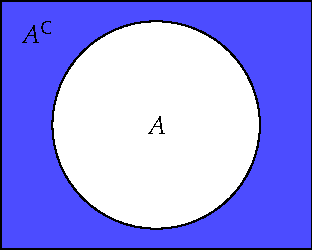
\includegraphics[width=\textwidth]{sets-05-venncomp}\\
$\comp A$: everything not in $A$\\[20pt]
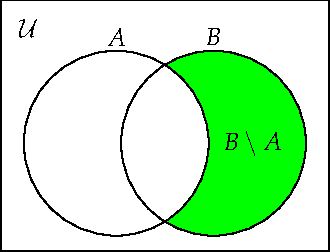
\includegraphics[width=\textwidth]{sets-06-vennrelcomp}\\
$B\setminus A$: everything in $B$ but not in $A$
\end{minipage}
\vspace{5pt}

\begin{example}
Let $\cU=\{1,2,3,4,5\}$, $A=\{1,2,3\}$, and $B=\{2,3,4\}$. Then
\[\comp A=\{4,5\},\qquad \comp B=\{1,5\},\qquad B\setminus A=\{4\},\qquad A\setminus B=\{1\}.\]
\end{example}
\vspace{3pt}


\noindent\begin{minipage}{0.62\textwidth}
Now we construct sets based on \emph{or} and \emph{and.}

\begin{defn}\label{defn:unionint}
The \emph{union} of $A$ and $B$ is the set
\[A\cup B=\{x\in\cU:x\in A\text{ or }x\in B\}.\]
The \emph{intersection} of $A$ and $B$ is the set
\[A\cap B=\{x\in\cU:x\in A\text{ and }x\in B\}.\]
We say that $A$ and $B$ are \emph{disjoint} if $A\cap B=\emptyset$.
\end{defn}
\end{minipage}\qquad
\begin{minipage}{0.33\textwidth}
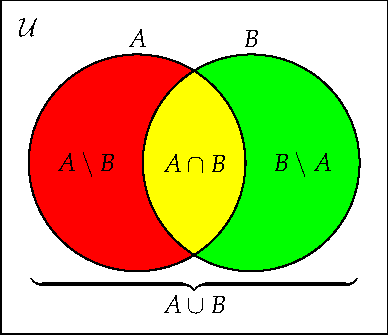
\includegraphics[width=\textwidth]{sets-04-vennunion}
\end{minipage}\\

\noindent In the Venn diagram, the sets $A$ and $B$ are again depicted as overlapping circles. Although it doesn't constitute a proof, the diagram makes it clear that
\[A=(A\setminus B)\cup (A\cap B)\quad\text{and}\quad B=(B\setminus A)\cup(A\cap B).\]

`Or' is used in the logical sense: $A\cup B$ is the collection of all elements that lie in $A$, in $B$, or in both.
Now observe the notational pattern: $\cup$ looks very similar to the logic symbol $\vee$ from Chapter \ref{sec:logic}. The symbols $\cap$ and $\wedge$ are also similar. This should help you remember which symbol to use when!

\begin{examples}
\item Let $\cU=\{$fish, dog, cat, hamster$\}$, $A=\{$fish, cat$\}$, and $B=\{$dog, cat$\}$. Then,
\[A\cup B=\{\text{fish, dog, cat}\},\qquad A\cap B=\{\text{cat}\}.\]
\item Using interval notation, let $\cU=[-4,5]$, $A=[-3,2]$, and $B=[-4,1)$. Then
\[\comp A=[-4,-3)\cup (2,5],\qquad \comp B=[1,5],\qquad B\setminus A=[-4,-3),\qquad A\setminus B=[1,2].\]
\vspace{-24pt}
\begin{center}
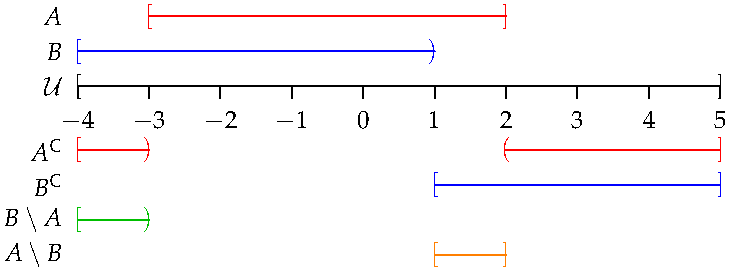
\includegraphics[width=0.7\textwidth]{sets-13-intervalex}
\end{center}\vspace{-13pt}
\item Let $A=(-\infty,3)$ and $B=[-2,\infty)$ in interval notation. Then $A\cup B=\R$ and $A\cap B=[-2,3)$.
\end{examples}

\noindent We didn't mention the universal set in the final example, though it seems reasonable to assume that $\cU=\R$. In practice $\mathcal U$ is rarely made explicit, and is often assumed to be the smallest suitable uncomplicated set. When dealing with sets of real numbers this typically means $\cU=\R$. In other situations $\cU=\Z$ or $\cU=\{0,1,2,3,\ldots,n-1\}$ might be more appropriate.\\

The next theorem comprises the basic rules of set algebra.

\begin{thm}\label{thm:setbasic}
Let $A,B,C$ be sets. Then:
\begin{enumerate}\setlength{\itemsep}{0pt}
\item $\emptyset\cup A=A$ \ and \ $\emptyset\cap A=\emptyset$.
\item $A\cap B\subseteq A\subseteq A\cup B$.
\item $A\cup B=B\cup A$ \ and \ $A\cap B=B\cap A$.
\item $A\cup (B\cup C)=(A\cup B)\cup C$ \ and \ $A\cap (B\cap C)=(A\cap B)\cap C$.
\item $A\cup A=A\cap A=A$.
\item $A\subseteq B\implies A\cup C\subseteq B\cup C$ \ and \ $A\cap C\subseteq B\cap C$.
\end{enumerate}
\end{thm}

\noindent You should be able to prove each of these properties directly from Definitions \ref{defn:subset} and \ref{defn:unionint}. Don't memorize the proofs: with a little practice working with sets, each of these results should feel completely obvious. It is more important that you are able to \emph{vizualize} the laws using Venn diagrams. A Venn diagram does not constitute a formal proof, though it is extremely helpful for clarification. Here we prove only second result: think about how the Venn diagram in Definition \ref{defn:unionint} illustrates the result. Some of the other proofs are in the Exercises.

\begin{proof}[Proof of 2.]
There are two results here: $A\cap B\subseteq A$ and $A\subseteq A\cup B$. We show each separately, along with some of our reasoning.
\begin{itemize}\setlength{\itemsep}{-2pt}
  \item[]Suppose that $x\in A\cap B$.\hfill(Must show $x\in A\cap B\Rightarrow x\in A$)
  \item[]Then $x\in A$ and $x\in B$.\hfill(Definition of intersection)
  \item[]But then $x\in A$, whence $A\cap B\subseteq A$\hfill(Definition of subset)
  \item[]Now let $y\in A$.\hfill(Must show $y\in A\Rightarrow y\in A\cup B$)
  \item[]Then `$y\in A$ or $y\in B$' is true, from which we conclude that $y\in A\cup B$.
  \item[]Thus $A\subseteq A\cup B$.\qedhere
\end{itemize}
\end{proof}

The following theorem describes how complements interact with other set operations.\\


\noindent\begin{minipage}{0.62\textwidth}
\begin{thmm}\label{thm:setcomp}
Let $A,B$ be sets. Then:
\begin{enumerate}\setlength{\itemsep}{0pt}
\item $\comp{(A\cap B)}=\comp A\cup \comp B$.
\item $\comp{(A\cup B)}=\comp A\cap \comp B$.
\item $\comp{(\comp A)}=A$.
\item $A\setminus B=A\cap\comp B$.
\item $A\subseteq B\iff \comp B\subseteq \comp A$.
\end{enumerate}
\end{thmm}
\end{minipage}\qquad
\begin{minipage}{0.33\textwidth}\centering
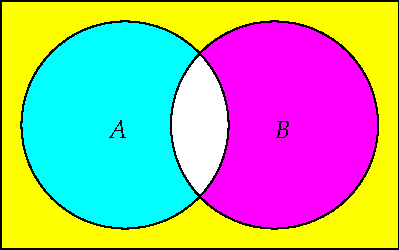
\includegraphics[width=\textwidth]{sets-08-venndemorgan}\\
$\comp{(A\cap B)}=\comp A\cup \comp B$
\end{minipage}\\[5pt]

\noindent Again: don't memorize these laws! Draw Venn diagrams to help with visualization. 

\begin{proof}[Proof of 1.]
We start by trying to show that the left hand side is a subset of the right hand side.
\begin{align*}
x\in\comp{(A\cap B)}&\implies x\notin A\cap B\\
&\implies x\text{ is not a member of \emph{both} $A$ and $B$}\\
&\implies x\text{ is not in \emph{at least one} of $A$ and $B$}\\
&\implies x\notin A\text{ or }x\notin B\\
&\implies x\in\comp A\text{ or }x\in\comp B\\
&\implies x\in\comp A\cup\comp B
\end{align*}
With a little thinking, we realize that all of the $\Longrightarrow$ arrows may be replaced with if and only if arrows $\Longleftrightarrow$ without compromising the argument. We've therefore shown that the sets $\comp{(A\cap B)}$ and $\comp A\cup \comp B$ have the same elements, and are thus equal.
\end{proof}

\noindent We were lucky with our proof. Showing that both sides are subsets of each other would have been tedious, but we found a quicker proof by carefully laying out one direction. This happens more often than you might expect. Just be careful: you can't always make conditional connectives biconditional.\\

\noindent Parts 1.\ and 2. of the theorem are known as \emph{De Morgan's laws}, just as the equivalent statements in logic: Theorem \ref{thm:demorgan}. Indeed, we could rephrase our proof in that language.

\begin{proof}[Alternative Proof of 1.]
\begin{align*}
x\in\comp{(A\cap B)}&\iff \neg[x\in A\cap B]\\
&\iff \neg[x\in A\ \text{ and }\  x\in B]\\
&\iff \neg[x\in A]\ \text{ or }\ \neg[x\in B]\tag*{(De Morgan's first law)}\\
&\iff x\in\comp A\ \text{ or }\ x\in\comp B\\
&\iff x\in\comp A\cup\comp B\tag*{\qedhere}
\end{align*}
\end{proof}

Finally, we have two results which describe the interaction of unions and intersections.\\

\noindent\begin{minipage}{0.65\textwidth}
\begin{thmm}[Distributive laws]\label{thm:setdist}
For any sets $A,B,C$:
\begin{enumerate}\setlength{\itemsep}{2pt}
\item $A\cap(B\cup C)=(A\cap B)\cup(A\cap C)$
\item $A\cup(B\cap C)=(A\cup B)\cap(A\cup C)$
\end{enumerate}
\end{thmm}

We prove only the second result. The method is the standard approach: show that each side is a subset of the other. We do both directions this time, though with a little work and the cost of some clarity, you might be able to slim down the proof. The Venn diagram on the right illustrates the second result: simply add the colored regions.
\end{minipage}\qquad
\begin{minipage}{0.28\textwidth}\centering
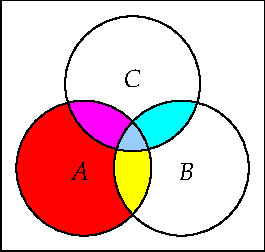
\includegraphics[width=\textwidth]{sets-07-venndist}
\end{minipage}\\


\begin{proof}
\begin{itemize}
  \item[($\subseteq$)] Let $x\in A\cup (B\cap C)$. Then $x\in A$ or $x\in B\cap C$. There are two cases:
  \begin{itemize}
    \item[(a)] If $x\in A$, then $x\in A\cup B$ and $x\in A\cup C$ by Theorem \ref{thm:setbasic}, part 2.
    \item[(b)] If $x\in B\cap C$, then $x\in B$ and $x\in C$. It follows that $x\in A\cup B$ and $x\in A\cup C$, again by Theorem \ref{thm:setbasic}.
  \end{itemize}
  In both cases $x\in (A\cup B)\cap(A\cup C)$.
  \item[($\supseteq$)] Let $y\in (A\cup B)\cap(A\cup C)$. Then $y\in A\cup B$ and $y\in A\cup C$. There are again two cases:
  \begin{itemize}
    \item[(a)] If $y\in A$, then we are done, for then $y\in A\cup (B\cap C)$.
    \item[(b)] If $y\notin A$, then $y\in B$ and $y\in C$. Hence $y\in B\cap C$. In particular $y\in A\cup (B\cap C)$.
  \end{itemize}
  In both cases $y\in A\cup (B\cap C)$.\qedhere
\end{itemize}
\end{proof}

\paragraph{Self-test Questions}

\begin{enumerate}
  \item The set operations of complement, union and intersection are based, respectively, on the logical constructions \underline{\phantom{not\quad}}, \underline{\phantom{or\quad}}, and \underline{\phantom{and\quad}}.
  \item The result $\comp{(A\cup B)}=\comp A\cap\comp B$ is one of \underline{\phantom{De Morgan's laws\qquad}}.
  \item True or false: if $A$ and $B$ are finite sets, then $A\cap B$ has strictly smaller cardinality than $A$.
  \item True or false: if $A$ is a finite set, then $\comp A$ is a finite set.
  \item True of false: if $A$ and $B$ are finite sets, then $\nm{A\cup B}\le\max(\nm A,\nm B)$.
\end{enumerate}

\subsection*{Exercises}

\begin{enumerate}\renewcommand{\labelenumi}{\thesubsection.\theenumi}
  \item Describe each of the following sets in as simple a manner as you can: e.g.,
  \[\{x\in\R:(x^2>4\text{ and } x^3<27)\text{ or } x^2=15\}=(-\infty,-2)\cup (2,3)\cup\{\sqrt{15}\}.\]
	\begin{enumerate}
	  	\item $\{x\in\R:x^2\neq x\}$
	  	\item $\{x\in\R:x^3-2x^2-3x\le 0\text{ or }x^2=4\}$
	  	\item $\{x^2\in\R:x \neq 1\}$
	  	\item $\{z\in\Z:z^2\text{ is even and $z^3$ is odd}\}$
		  \item $\{y\in 3\Z+2:y^2\equiv 1\pmod 3\}$
		\end{enumerate}
  
  \item Let $A=\{1,3,5,7,9,11\}$ and $B=\{1,4,7,10,13\}$. What are the following sets?
    \begin{enumerate}
	  	\item $A\cap B$
	  	\item $A\cup B$
	  	\item $A\setminus B$
	  	\item $(A\cup B)\setminus (A\cap B)$
		\end{enumerate}
	
  	
  \item Let $A\subseteq\R$, and let $x\in\R$. We say that the point $x$ is \emph{far away} from the set $A$ if and only if:
  \[\exists d>0\colon\text{ No element of $A$ belongs to the set $[x-d,x]$}.\]
	Equivalently, $A\cap[x-d,x]=\emptyset$. 
	If this does not happen, we say that $x$ is \emph{close to} $A$.
  	\begin{enumerate}
			\item Draw a picture of a set $A$ and an element $x$ such that is  \emph{far away} from $A$. 
			\item Draw a picture of a set $A$ and an element  $x$  such that $x$ is \emph{close} to $A$.
			\item Compute the definition of ``$x$ is close to $A$''. [So negate ``$x$ is far away from $A$''.]
			\item Let $A=\{1,2,3\}$. Show that $x=4$ is \emph{far away} from $A$, by using definitions.
			\item Let $A=\{1,2,3\}$. Show that $x=1$ is \emph{close} to  $A$, by using definitions.
			\item Show that if $x\in A$, then $x$ is \emph{close} to $A$.
			\item Let $A$ be the open interval $(a,b)$. Is the end-point $a$ \emph{far away} from $A$?  What about the end-point $b$?
  	\end{enumerate}
  	
	\item Consider Theorems \ref{thm:setbasic} and \ref{thm:setdist}. In all seven results, replace the symbols in the first row of the following table with those in the second. Which of the results seem familar? Which are false?
\[\begin{array}{c|c|c|c|c}
\emptyset&A,B,C\text{ sets}&\cup&\cap&\subseteq\\\hline
0&A,B,C\in\N_0&+&\cdot&\le
\end{array}\]

	\item Prove that $B\setminus A=B\iff A\cap B=\emptyset$.
	
	\item Practice your proof skills by giving formal proofs of the following results from Theorems \ref{thm:setbasic} and \ref{thm:setcomp}. With practice you should be able to prove \emph{all} of parts of these theorems (and of Theorem \ref{thm:setdist}) these \emph{without} looking at the arguments in the notes!
	\begin{enumerate}
	  \item $\emptyset\cap A=\emptyset$.
		\item $A\cap (B\cap C)=(A\cap B)\cap C$.
		\item $\comp{(\comp A)}=A$.
		\item $A\subseteq B\iff \comp B\subseteq \comp A$.
	\end{enumerate}

	\item Write out a formal proof of the set identity
	\[A=(A\setminus B)\cup (A\cap B)\]
	by showing that each side is a subset of the other. Now repeat your argument using only results from set algebra (Theorems \ref{thm:setcomp} and \ref{thm:setdist}).
\end{enumerate}
\newpage


\subsection{Introduction to Functions}\label{sec:func1}

You have been using functions for a long time. A formal definition in terms of relations will be given in Section \ref{sec:func2}. For the present, we will just use the following.

\begin{defn}
Let $A$ and $B$ be sets. A \emph{function from $A$ to $B$} is a rule $f$ that assigns one (and only one) element of $B$ to each element of $A$.\\
The \emph{domain} of $f$, written $\dom(f)$, is the set $A$. The \emph{codomain} of $f$ is the set $B$.\\
The \emph{range} or \emph{image} of $f$, written $\range(f)$ or $\operatorname{Im}(f)$, is the subset of $B$ consisting of all the elements assigned by the rule $f$.
\end{defn}

\noindent You can think of the domain of $f$ as the set of all inputs for the function, and the range of $f$ as the set of all outputs. The codomain is the set of all potential values the function may take (of course, only the values in the range are actually achieved).

\subsubsection*{Notation}

If $f$ is a function from $A$ to $B$ we write $f:A\to B$.\\
If $a\in A$, we write $b=f(a)$ for the the element of $B$ assigned to $a$ by the function $f$.\\
We can also write $f:a\mapsto b$, which is read `$f$ maps $a$ to $b$.'\\
If $U$ is a subset of $A$ then the \emph{image} of $U$ is the following subset of $B$,\vspace{-4pt}
\[f(U)=\{f(u)\in B:u\in U\}.\vspace{-5pt}\]
The image of $A$ is precisely the range of $f$, hence the notation $\operatorname{Im}(f)$,\vspace{-4pt}
\[f(A)=\range(f)=\operatorname{Im}(f)=\{f(a)\in B:a\in A\}.\vspace{-2pt}\]


\begin{center}
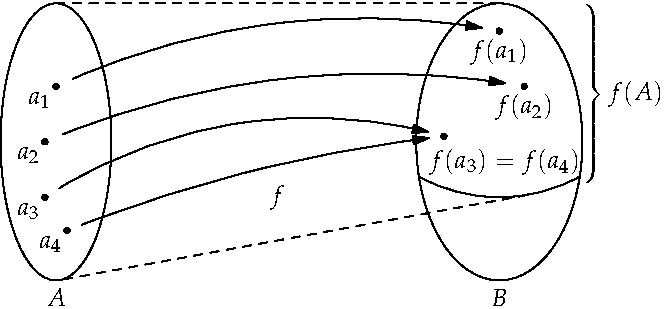
\includegraphics[width=0.6\textwidth]{sets-16-funcdef}
\end{center}



\noindent\begin{minipage}{0.62\textwidth}
		For simple real-valued functions, the domain and range are easily seen in a graph. For instance if $f:[-3,2)\to\R$ is the square function
		\[f:x\mapsto x^2,\]
		then we have $\dom(f)=[-3,2)$ and $\range(f)=[0,9]$, as seen in the picture. We could also calculate other images, for example,
  	\[f\bigl([-1,2)\bigr)=[0,4).\]
  \end{minipage}\hfill
  \begin{minipage}{0.33\textwidth}
  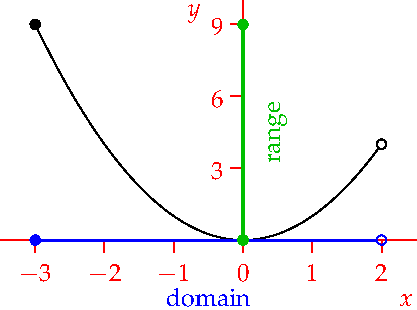
\includegraphics[width=\textwidth]{sets-10-rangedom}
  \end{minipage}\\
  
\noindent For most functions we will not be able to sketch a graph. Here are several examples where a graph is either unhelpful, or simply impossible to draw!
  
\begin{examples}
  \item Define $f:\Z\to\{0,1,2\}$ by $f:n\mapsto n^2\pmod 3$, where we take the remainder of $n^2$ modulo 3. Clearly $\dom(f)=\Z$, but what is the range? Trying a few examples, we see the following:
  \[\begin{array}{c|ccccccccccc}
  n&0&1&2&3&4&5&6&7&8&9&10\\\hline
  f(n)&0&1&1&0&1&1&0&1&1&0&1
  \end{array}\]
  It looks like the range is simply $\{0,1\}$. We have already proved this fact in Theorem \ref{thm:sqmod3}, although a faster proof can now be given by appealing to modular arithmetic (Section \ref{sec:cong}).
  \begin{itemize}\setlength{\itemsep}{0pt}
    \item[] If $n\equiv 0$, then $n^2\equiv 0\pmod 3$.
    \item[] If $n\equiv 1$, then $n^2\equiv 1\pmod 3$.
    \item[] If $n\equiv 2$, then $n^2\equiv 4\equiv 1\pmod 3$.
  \end{itemize}
  Thus $n^2\equiv 0,1\pmod 3$, and $\range(f)=\{0,1\}$.
  \item\label{ex:functmod1} Let $A=\{0,1,2,\ldots,9\}$ be the set of remainders modulo 10 and define $f:A\to A$ by $f:n\mapsto 3n\pmod{10}$. To help understand this function, list the elements: the domain only has 10 elements after all.
  \[\begin{array}{c|cccccccccc}
  n&0&1&2&3&4&5&6&7&8&9\\\hline
  f(n)&0&3&6&9&2&5&8&1&4&7
  \end{array}\]
  It should be obvious that $\range(f)=A$.
  \item\label{ex:functmod2} With the same notation as the previous example, let $g:A\to A:n\mapsto 4n\pmod{10}$. Now we have the following table:
  \[\begin{array}{c|cccccccccc}
  n&0&1&2&3&4&5&6&7&8&9\\\hline
  g(n)&0&4&8&2&6&0&4&8&2&6
  \end{array}\]
  with $\range(g)=\{0,2,4,6,8\}$.
  \item Let $A=\{1,2,3,4,5\}$ and let $B=\{$two-element subsets of $A\}$. We define
  \[f:A\to B:a\mapsto\begin{cases}
  \{a,a+1\}&\text{if }a\neq 5,\\
  \{5,1\}&\text{if }a=5.
  \end{cases}\]
  This is tricky to read, since $B$ is a set of sets. You should be able to convince yourself that
  \[\range(f)=\big\{\{1,2\},\{2,3\},\{3,4\},\{4,5\},\{5,1\}\big\}\]
  and, for example, that
  \[f\big\{1,4\big\}=\big\{f(1),f(4)\big\}=\big\{\{1,2\},\{4,5\}\big\}\]
\end{examples}

\subsubsection*{Injections, surjections and bijections}

\begin{defn}\label{defn:11}
A function $f:A\to B$ is \emph{1--1} (one-to-one), \emph{injective}, or an \emph{injection} if it never takes the same value twice. Equivalently,\footnote{This is the contrapositive: if $f$ never takes the same value twice, then $\forall a_1, a_2\in A$ we have $a_1\neq a_2\implies f(a_1)\neq f(a_2)$.}
\[\forall a_1,a_2\in A,\ f(a_1)=f(a_2)\implies a_1=a_2.\]
$f:A\to B$ is \emph{onto}, \emph{surjective}, or a \emph{surjection} if it takes every value in the codomain: i.e., $B=\range(f)$. Equivalently,\footnote{This is the statement $B\subseteq\range(f)$. The opposite inclusion $\range(f)\subseteq B$ is true for \emph{any} function.}
\[\forall b\in B,\ \exists a\in A\text{ such that }f(a)=b.\]
$f:A\to B$ is \emph{invertible}, \emph{bijective}, or a \emph{bijection} if it is both injective and surjective.
\end{defn}

\noindent Since the definitions of injective and surjective are both `for all' statements, to show that a function is \emph{not injective} or \emph{not surjective} you will need \emph{counterexamples.} For instance, consider the quadratic function $f:[-3,2)\to\R:x\mapsto x^2$ seen above. It is straightforward to see that $f$ is neither injective nor surjective. Indeed we have the following counterexamples:
		\begin{itemize}%\setlength\itemsep{0pt}
  	  \item $f(-1)=f(1)$. If $f$ were injective, the values at 1 and $-1$ would have to be different.
  	  \item $81\in\R$, yet there is no $x\in[-3,2)$ such that $f(x)=81$. Thus $f$ is not surjective.
		\end{itemize}
With a small change to either the domain or codomain, we can easily create an injective or a surjective function. For instance we can shrink the domain to obtain two injective functions:
\[g:[0,2)\to\R:x\mapsto x^2\quad\text{and}\quad h:[-3,0]\to\R:x\mapsto x^2\]
\begin{center}
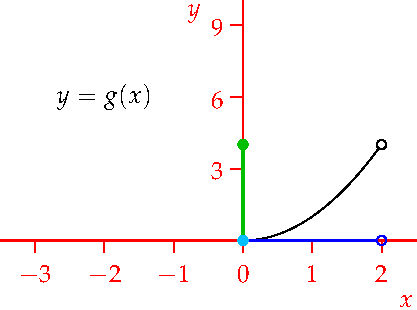
\includegraphics[width=0.4\textwidth]{sets-18-rangedom2}
\qquad\qquad\qquad
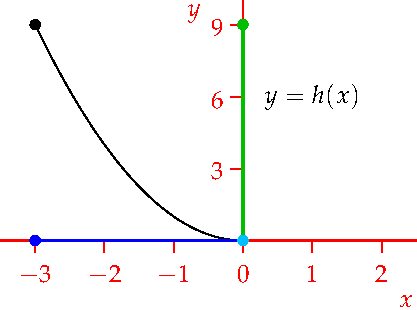
\includegraphics[width=0.4\textwidth]{sets-19-rangedom3}
\end{center}
To see this, note that
\[g(x_1)=g(x_2)\implies x_1^2=x_2^2\implies x_1=\pm x_2\implies x_1=x_2\]
since both must be non-negative. The argument for $h$ is similar.\\
By shrinking the codomain to equal the range we immediately create a surjective function:
\[j:[-3,2)\to [0,9]:x\mapsto x^2\]


Now consider the examples on page \pageref{ex:functmod1}. The details are provided for example 1. For the others, make sure you understand why the answer is correct. 
\begin{examples}
  \item $f:\Z\to\{0,1,2\}:n\mapsto n^2\pmod 3$ is neither injective nor surjective.
  	\begin{itemize}
  	  \item If $f$ were injective, then we could not have $f(1)=f(2)$.
  	  \item 2 is in the codomain $\{0,1,2\}$ of $f$, yet $2\notin\range(f)$, so $f$ is not surjective.
		\end{itemize}
  \item This is a bijection. Indeed $f$ is  a \emph{permutation,} a bijection from a set onto itself. To see injectivity, note that in the table
  \[\begin{array}{c|cccccccccc}
  n&0&1&2&3&4&5&6&7&8&9\\\hline
  f(n)&0&3&6&9&2&5&8&1&4&7
  \end{array}\]
  none of the values in the second row appears more than once. For surjectivity, observe that every element in the codomain $\{0,1,2,\ldots,9\}$ appears \emph{at least} once in the second row. Being bijective means that each element of the codomain appears \emph{exactly once.}
  \item Neither injective, nor surjective.
  \item Injective, but not surjective.
\end{examples}


Here is a more complicated example.
\begin{example}
Prove that $f:\R\setminus\{1\}\to\R\setminus\{2\}$ defined by $f(x)=2+\frac 1{1-x}$ is bijective.\\[2pt]

\noindent\begin{minipage}{0.6\textwidth}
		\begin{itemize}
  	  \item[](Injectivity)\quad Suppose that $x_1$ and $x_2$ are in $\R\setminus\{1\}$, and $f(x_1)=f(x_2)$. Then
			\[2+\frac 1{1-x_1}=2+\frac 1{1-x_2}.\]
			A little elementary algebra shows that $x_1=x_2$, whence $f$ is injective.
  	  \item[](Surjectivity)\quad Let $y\in\R\setminus\{2\}$ and define $x=1-\frac 1{y-2}$. This makes sense since $y\neq 2$. Then
  	  \[f(x)=2+\frac 1{1-(1-\frac 1{y-2})}=y\]
  	  whence $f$ is surjective.
		\end{itemize}
  \end{minipage}\qquad
  \begin{minipage}{0.35\textwidth}
  	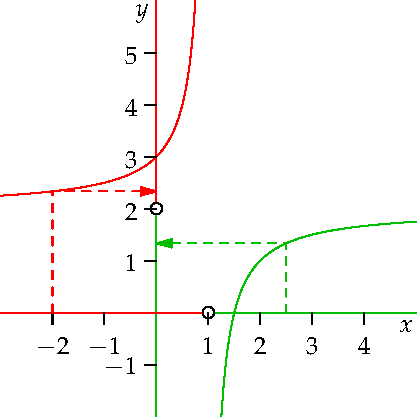
\includegraphics[width=\textwidth]{sets-09-bij}
  \end{minipage}\\[2pt]
The graphic is colored so that you can see how the different parts of the range and domain correspond. The argument for surjectivity is sneaky: how did we know to choose $x=1-\frac 1{y-2}$? The answer is scratch work: just solve $y=2+\frac 1{1-x}$ for $x$. Essentially we've shown that $f$ has the inverse function $f^{-1}(x)=1-\frac 1{x-2}$.
\end{example}

\begin{aside}
\noindent{\bf Inverse Functions}

The word \emph{invertible} is a synonym for bijective because bijective functions really have inverses! Indeed, suppose that $f:A\to B$ is bijective. Since $f$ is surjective, we know that $B=\range(f)$ and so every element of $B$ has the form $f(a)$ for some $a\in A$. Moreover, since $f$ is injective, the $a$ in question is unique. The upshot is that, when $f$ is bijective, we can construct a new \emph{function}
\[f^{-1}:B\to A:f(a)\mapsto a.\]
This may appear difficult at the moment but we will return to it in Chapter \ref{sec:relations}.

Instead, recall that in Calculus you saw that any injective function has an inverse. How does this fit with our definition? Consider, for example, $f:[0,2]\to\R:x\mapsto x^4$. This is injective but not surjective. To fix this, simply define a new function with the same formula but with codomain equal to the range of $f$. We obtain the bijective function
\[g:[0,2]\to[0,16]:x\mapsto x^4,\]
with inverse
\[g^{-1}:[0,16]\to[0,2]:x\mapsto \sqrt[4]{x}.\]
In Calculus we didn't nitpick like this and would simply go straight to $f^{-1}(x)=\sqrt[4]{x}$.\\[5pt]
In general, if $f:A\to B$ is any injective function, then $g:A\to f(A):x\mapsto f(x)$ is automatically bijective, since we are forcing the codomain of $g$ to match its range.
\end{aside}

\subsubsection*{Functions and Cardinality}

Injective and surjective functions are intimately tied to the notion of cardinality. Indeed, in Chapter \ref{sec:card}, we will use such functions to give a \emph{definition} of cardinality for infinite sets. For the present we stick to finite sets. 

\begin{thm}\label{thm:finitecard}
Let $A$ and $B$ be finite sets. The following are equivalent:
\begin{enumerate}\setlength{\itemsep}{0pt}
  \item $\nm A\le\nm B$.
  \item $\exists f:A\to B$ injective.
  \item $\exists g:B\to A$ surjective.
\end{enumerate}
\end{thm}

\noindent\begin{minipage}{0.8\textwidth}
Read the theorem carefully. It is simply saying that, of the three statements, if \emph{any} one is true then \emph{all} are true. Similarly, if one is false then so are the others. It might appear that we require six arguments! Instead we illustrate an important technique: when showing that multiple statements are equivalent, it is enough to prove in a circle. For instance, if we prove the three implications indicated in the picture, then $\circimp 13$ will be true because \emph{both} \circimp 12 and \circimp 23 are true.\\
\end{minipage}\qquad
\begin{minipage}{0.15\textwidth}
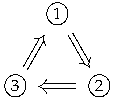
\includegraphics[width=\textwidth]{sets-14-circlearg}
\end{minipage}

\noindent More generally, to show that $n$ statements are equivalent, only $n$ arguments are required.\pagebreak

\noindent The proof may appear very abstract, but it is motivated by two straightforward pictures. Don't be afraid to use pictures to illustrate your proofs if it's going to make them easier to follow! If $\nm A=m$ and $\nm B=n$, then the two functions  can be displayed pictorially. Refer back to these pictures as you read through the proof.
\begin{center}
\begin{tabular}{c@{\hspace{1cm}}c}
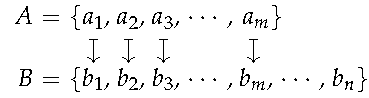
\includegraphics[scale=0.9]{sets-11-finiteinj}&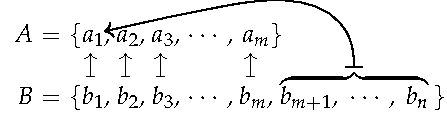
\includegraphics[scale=0.9]{sets-12-finiteinj}\\
The function $f$&The function $g$
\end{tabular}
\end{center}

\begin{proof}
The proof relies crucially on the fact that $A,B$ are finite. Suppose that $\nm A=m$ and $\nm B=n$ throughout and list the elements of $A$ and $B$ as,
\[A=\{a_1,a_2,\ldots,a_m\},\qquad\qquad B=\{b_1,b_2,\ldots,b_n\}.\]
\noindent\begin{tabular}{@{}p{0.13\textwidth}@{}p{0.87\textwidth}@{}}
$\bigl(\circimp 12\bigr)$&Assume that $m\le n$. Define $f:A\to B$ by $f(a_k)=b_k$. This is injective since the elements $b_1,\ldots,b_m$ are distinct.\\
$\bigl(\circimp 23\bigr)$&Suppose that $f:A\to B$ is injective. Without loss of generality we may assume that the elements of $A$ and $B$ are labeled such that $f(a_k)=b_k$. Now define $g:B\to A$ by
  \[g(b_k)=\begin{cases}
  a_k&\text{ if }k\le m,\\
  a_1&\text{ if }k>m.
  \end{cases}\]
  Then $g$ is surjective since every element $a_k$ is in the image of $g$.\\
$\bigl(\circimp 31\bigr)$&Finally suppose that $g:B\to A$ is surjective. Without loss of generality we may assume that $a_k=g(b_k)$ for $1\le k\le m$. Thus $n\ge m$.\qedhere  
\end{tabular}
\end{proof}

\noindent It is worth noting in the proof of $\bigl(\circimp 31\bigr)$ that the elements $b_{m+1},\ldots,b_n$ may be mapped \emph{anywhere,} not just to $a_1$ as suggested in the picture above.

\noindent If you read the proof carefully, it should be clear that when $m=n$, the function $f$ is actually a \emph{bijection} (with inverse $f^{-1}=g$).


\begin{cor}\label{cor:finitecard}
If $A,B$ are finite sets, then $\nm A=\nm B\iff\exists f:A\to B$ bijective.
\end{cor}

\begin{proof}
Suppose that $m=n$. The argument \circimp 12 creates an injective function $f:A\to B$. However every element $b_k\in B$ is in the image of $f$, so this function is also surjective. Hence $f$ is a bijection.\\
Conversely, if $f:A\to B$ is a bijection, then it is injective, whence $m\le n$. It is also surjective, from which $n\le m$. Therefore $m=n$. 
\end{proof}\pagebreak


\subsubsection*{Composition of functions}

Finally, we consider composing function and, more particularly, how injectivity and surjectivity interact with composition.

\begin{defn}
Suppose that $f:A\to B$ and $g:B\to C$ are functions. The \emph{composition} $g\circ f:A\to C$ is the function defined by $(g\circ f)(a)=g(f(a))$.
\end{defn}
Note the order: to compute $(g\circ f)(x)$, you apply $f$ first, then $g$.

\begin{center}
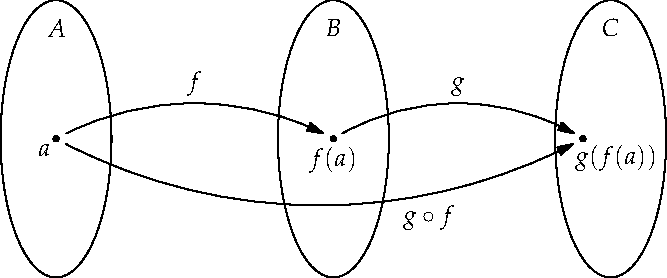
\includegraphics[width=0.65\textwidth]{sets-15-setcomp}
\end{center}

\begin{example}
If $f(x)=x^2$ and $g(x)=\frac 1{x-1}$, then
\[(g\circ f)(x)=\frac 1{x^2-1},\quad\text{and}\quad(f\circ g)(x)=\frac 1{(x-1)^2}.\]
You should be extra careful of ranges and domains when composing functions. The domain and range are not always explicitly mentioned, and at times some restriction of the domain is implied. In this example, you might assume that $\dom(f)=\R$ and $\dom(g)=\R\setminus\{1\}$. This is perfectly good if we are considering $f$ and $g$ separately. However, it should be clear from the formulæ that the implied domains of the compositions are,
\[\dom(g\circ f)=\R\setminus\{\pm 1\},\quad\text{and}\quad\dom(f\circ g)=\R\setminus\{1\}.\]
\end{example}

Our first two results on composing injective and surjective functions is easy to remember.

\begin{thm}\label{thm:compinjsurj}
Let $f:A\to B$ and $g:B\to C$ be functions. Then:
\begin{enumerate}
  \item If $f$ and $g$ are injective, then $g\circ f$ is injective.
  \item If $f$ and $g$ are surjective, then $g\circ f$ is surjective.
\end{enumerate}
It follows that the composition of bijective functions is also bijective.
\end{thm}

\begin{proof}
\begin{enumerate}
  \item Suppose that $f$ and $g$ are injective and let $a_1,a_2\in A$ satisfy $(g\circ f)(a_1)=(g\circ f)(a_2)$. We are required to show that $a_1=a_2$. However,
  \begin{align*}
  (g\circ f)(a_1)=(g\circ f)(a_2)&\implies g\big(f(a_1)\big)=g\big(f(a_2)\big)\\
  &\implies f(a_1)=f(a_2)\tag*{(since $g$ is injective)}\\
  &\implies a_1=a_2\tag*{(since $f$ is injective)}\\[-25pt]
  \end{align*}\qedhere
%   \item Now suppose that $f$ and $g$ are surjective. Let $c\in C$. We are required to show that $\exists a\in A$ such that $(g\circ f)(a)=c$.\\
%   Since $g$ is surjective, $\exists b\in B$ such that $g(b)=c$.\\
%   Similarly, since $f$ is surjective, $\exists a\in A$ such that $f(a)=b$.\\
%   Together we have $(g\circ f)(a)=g(f(a))=c$, as required.
\end{enumerate}
\end{proof}

\noindent Part 2 is in the Exercises. It is interesting to observe that the converse of this theorem is \emph{false.} Assuming that a composition is injective or surjective only forces \emph{one} of the original functions to be so.

\begin{thm}
Suppose that $f:A\to B$ and $g:B\to C$ are functions.
\begin{enumerate}
  \item If $g\circ f$ is injective, then $f$ is injective.
  \item If $g\circ f$ is surjective, then $g$ is surjective.
\end{enumerate}
\end{thm}

\noindent Before showing the proof, consider the following representation of two functions $f$ and $g$ which simultaneously illustrate both parts of the theorem. It should be clear that $g\circ f$ is \emph{bijective,} $f$ is \emph{only injective,} and $g$ is \emph{only surjective.}

\begin{center}
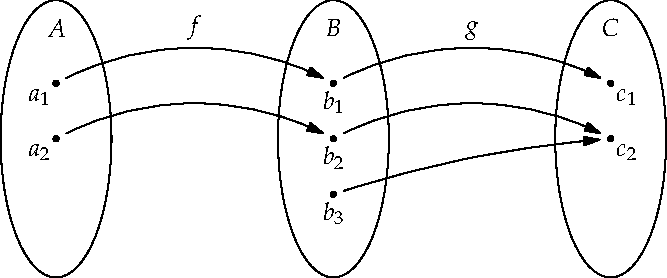
\includegraphics[width=0.65\textwidth]{sets-17-injcomp}
\end{center}

\noindent Here is a formulaic example of the same thing. Make sure you're comfortable with the definitions and draw pictures or graphs to help make sense of what's going on.
\begin{gather*}
f:[0,2]\to[-4,4]:x\mapsto x^2\tag*{(injective only)}\\[5pt]
g:[-4,4]\to [0,16]:x\mapsto x^2\tag*{(surjective only)}\\[5pt]
g\circ f:[0,2]\to[0,16]:x\mapsto x^4\tag*{(bijective!)}
\end{gather*}\pagebreak


\noindent This time we leave part 1 of the proof for the Exercises.
\begin{proof}
\begin{enumerate}\setcounter{enumi}{1}
%   \item Suppose that $f(a_1)=f(a_2)$. Then $(g\circ f)(a_1)=(g\circ f)(a_2)$. Since $g\circ f$ is injective we conclude that $a_1=a_2$, whence $f$ is injective.\qedhere
  \item Let $c\in C$ and assume that $g\circ f$ is surjective. We wish to prove that $\exists b\in B$ such that $g(b)=c$.\\
  Since $g\circ f$ is surjective, $\exists a\in A$ such that $(g\circ f)(a)=c$. But this says that
  \[g(f(a))=c.\]
  Hence $b=f(a)$ is an element of $B$ for which $g(b)=c$. Thus $g$ is surjective.\qedhere
\end{enumerate}
\end{proof}

\paragraph{Self-test Questions}

	\begin{enumerate}
    \item $f:A\to B$ is \emph{injective} if \underline{\phantom{$f(a_1)=f(a_2)\implies a_1=a_2$\qquad\qquad}}
    \item $f:A\to B$ is \emph{surjective} if \underline{\phantom{$\forall b\in B,\exists a\in A:f(a)=b$\qquad\qquad}}
    \item If $f\circ g$ is bijective, which of the following \emph{must} be true?
    \begin{itemize}
      \item $f$ is injective.
      \item $g$ is injective.
      \item $f$ is surjective. 
      \item $g$ is surjective.
    \end{itemize}
    \item True or false: We can always make a function surjective by making its domain smaller.
    \item True or false: If $A$ is a subset of $B$ then there exists an injective function $f:A\to B$.
  \end{enumerate}

\subsection*{Exercises}

\begin{enumerate}\renewcommand{\labelenumi}{\thesubsection.\theenumi}
  \item For each of the following functions $f:A\to B$ determine whether $f$ is injective, surjective or bijective. Prove your assertions.
  \begin{enumerate}
    \item $f:[0,3]\to\R$ where $f(x)=2x$.
    \item $f:[3,12)\to[0,3)$ where $f(x)=\sqrt{x-3}$.
    \item $f:(-4,1]\to(-5,-3]$ where $f(x)=-\sqrt{x^2+9}$.
  \end{enumerate}
  
  \item Suppose that $f:[-3,\infty)\to[-8,\infty)$ and $g:\R\to\R$ are defined by
	\[f(x)=x^2+6x+1,\qquad\qquad g(x)=2x+3.\]
	Compute $g\circ f$ and show that $g\circ f$ is injective.
  
  \item Find:
		\begin{enumerate}
			\item A set $A$ so that the function $f:A\to\R:x\mapsto\sin x$ is injective.
			\item A set $B$ so that the function $f:\R\to B:x\mapsto\sin x$ is surjective.
		\end{enumerate}


  \item (\emph{If you did Exercise \hyperref[ex:decreasing]{\ref*{sec:quant}.\ref*{ex:decreasing}} you should find this easy}) Let $X$ be a subset of $\R$. A function $f:X\to\R$ is \emph{strictly increasing} if 
	\[\forall \,a,\, b \in X,\quad a<b \Longrightarrow f(a)<f(b).\]
	For example, the function $f \colon [0,\,\infty)\to \R, \,x \mapsto x^2$  is increasing because 
	\[\forall a,\,b \in  [0,\,\infty) , \quad a<b \Longrightarrow f(a) = a^2< b^2=f(b).\]
		\begin{enumerate}
	  	\item Give another example of a function that is increasing. Draw its graph, and prove that  the function is increasing.  
	  	\item By negating the above definition, state what it means for a function \emph{not to be strictly increasing.} 
	  	\item Give an example of a function that is \emph{not} strictly increasing. Draw its graph, and prove that the function is not strictly increasing.  
	  	\item Let $f,\,g:\R\to\R$ be strictly increasing. Prove or disprove: The function $h=f+g$ is strictly increasing. Note that the formula for $h$ is $h(x)=f(x)+g(x)$.
		\end{enumerate}	
		
  \item You may assume that $g:[2,\infty)\to\R:x\mapsto \sqrt{x^3-8}$ is an injective function. Find a function $f:\R\to\R$ which is \emph{not injective,} but for which the composition $f\circ g:[2,\infty)\to\R$ \emph{is injective.} Justify your answer.

  \item A function $f:\R\to\R$ is \emph{even} if 
	\[\forall\,x\in\R,\ f(-x)=f(x).\]
	For example, the function $f:\R\to\R,\,x\mapsto x^2$ is even because 
	\[\forall\, x\in\R,\ f(-x)=(-x)^2= x^2=f(x).\]
	Note that $f$ is even if and only if the graph of $f$ is symmetric with respect to the $y$ axis. 
		\begin{enumerate}
	  	\item Give an example of a function that is even.  Draw its graph, and prove that  the function is even.
	  	\item Define what it means for a function \emph{not to be even}, by negating the definition above. 
	  	\item Give an example of a function that is \emph{not} even. Draw its graph, and prove that  the function is not even. 
	  	\item Prove or disprove: for every  $f ,\,g\colon \R \to \R$ even, the composition $ h= f\circ g$ is even. Here $h$ is the function mapping $x$ to $f(g(x))$.
		\end{enumerate}
	
  \item Define $f:(-\infty,0]\to\R$ and $g:[0,\infty)\to\R$ by
  \[f(x)=x^2,\qquad g(x)=\begin{cases}
  \frac{x}{1-x}&x<1,\\
  1-x&x\ge 1.
  \end{cases}\]
  Does $g\circ f$ map $(-\infty,0]$ onto $\R$? Justify your answer.\pagebreak
  
  \item Express, using quantifiers, what it means for a function to be
  \begin{enumerate}
    \item Not injective.
    \item Not surjective.
  \end{enumerate}
	
  \item Prove that the composition of two surjective functions is surjective.
  
  \item Suppose that $g\circ f$ is injective. Prove that $f$ is injective.
  
  \item In the proof of Theorem \ref{thm:finitecard} we twice invoked \emph{without loss of generality.} In both cases explain why the phrase applies.
  
  \item\label{ex:kfunc} Recall Examples \ref{ex:functmod1} and \ref{ex:functmod2} on page \pageref{ex:functmod1}.
  \begin{enumerate}
    \item Consider the nine functions $f_k:A\to A:x\mapsto kx\pmod{10}$, where $k=1,2,\ldots,9$. Find the range of $f_k$ for each $k$. Can you find a relationship between the cardinality of $\range(f_k)$ and $k$?
		\item More generally, let $A=\{0,1,2\ldots,n-1\}$ be the set of remainders modulo $n$. If $f_k:A\to A:x\mapsto kx\pmod n$, conjecture a relationship between $\nm{\range(f_k)}$, $k$ and $n$. You don't need to prove your assertions.
  \end{enumerate}
\end{enumerate}